% Pour toute question sur l'utilisation de cette classe, écrivez à jerome.soucy(at)ulaval.ca
% Nécessite la classe Evaluation.sty dans le même dossier ou dans le PATH de votre système
% Nécessite le fichier logo_ul.pdf dans le même dossier un dans le PATH de votre système
\def\Ponderation{35}
\def\SigleNumero{STT-1000}
\def\NomCours{Probabilités et statistique}
\def\DateEvaluation{2 mars 2023}
\def\HeureEvaluation{18h30 à 21h20}
\def\Session{Été 2021}
\def\NomEvaluation{Examen 1}

% Ne rien mettre entre les accolades si l'enseignant (ou l'enseignante) est aussi le coordonnateur (ou la coordonnatrice)
\def\Coordonnatrice{}
\def\Coordonnateur{}

% Ne rien mettre entre les accolades s'il y a plus d'une section
\def\Enseignant{}
\def\Enseignante{}

% Ne rien mettre entre les accolades s'il s'agit d'un cours à section unique
% Mettre le nom de chacun des enseignants et enseignantes entre les accolades
% Une case à cocher sera générée pour chacune des sections
\def\SectionA{Lajmi Lakhal-Chaieb}
\def\SectionB{Julien Miron}
\def\SectionC{}
\def\SectionD{}


\def\Directives{
\begin{enumerate}
\item Matériel autorisé:
\begin{itemize}
\item Calculatrice scientifique {\bf autorisée par la faculté des sciences et de génie};
\item Le feuillet de formules fourni avec l'examen. Celui-ci inclut la table de la loi normale. Veuillez ne rien écrire sur le feuillet de formules.
\end{itemize}
\item Assurez-vous que cette évaluation comporte \numquestions ~questions réparties sur \numpages{}~pages, pour un total de \numpoints{}~points/.\
\item \textbf{Veuillez ne pas dégrafer votre examen.}
\item Ajoutez vos initiales dans le bas de chaque page de l'examen.
\item Veuillez déposer votre carte d'identité \textbf{admise} avec photo sur votre bureau.\
\item Vous devez\textbf{ justifier votre réponse} par une démarche claire, sauf pour les questions à choix de réponse.\
\item Le verso des feuilles peut être utilisé comme brouillon, \textbf{mais ne sera pas corrigé}. Attention à ne rien dégrafer.
\end{enumerate}
}

% Veuillez indiquer le type d'évaluation entre crochets
% Examen : option à choisir pour un examen présentiel qui sera corrigé de manière classique. Un tableau des points sera affiché sur la page couverture.
% Gradescope : option à choisir pour un examen qui sera corrigé via Gradescope. Aucun tableau de pointage n'apparaîtra et il y a quelques différences au niveau de la mise en page
% TPS :
% TPF :
% Devoir :
\documentclass{Evaluation}
\usepackage{multicol,graphicx}

\printanswers

\begin{document}

\newpage
%%%%%%%%%%%%%%%% QUESTION %%%%%%%%%%%%%%%%
\begin{questions}
\question[5] Soient $A$ et $B$ deux événements de $\mathcal{U}$ tels que 
\begin{itemize}
\item $\mathbb{P}(\overline{A \cup B})=0.4$
\item $\mathbb{P}(A \cap \overline{B})=0.2$
\item $\mathbb{P}(\overline{A}\cap B)=0.1$
\end{itemize}
Calculer $\mathbb{P}(A \cap B)$.

\begin{solution}
On sait que $\mathbb{P}(\overline{A \cup B}) = 0{,}4$, donc $\mathbb{P}(A \cup B) = 1 - 0{,}4 = 0{,}6$.

Or, l'union se décompose en trois parties disjointes :
$$\mathbb{P}(A \cup B) = \mathbb{P}(A \cap \overline{B}) + \mathbb{P}(\overline{A} \cap B) + \mathbb{P}(A \cap B)$$
Donc
$$0{,}6 = 0{,}2 + 0{,}1 + \mathbb{P}(A \cap B)$$
$$\mathbb{P}(A \cap B) = 0{,}3$$
\end{solution}

\vspace{7cm}
\question[5] Soient $A$, $B$ et $C$ trois événements de $\mathcal{U}$ tels que 
\begin{itemize}
\item $\mathbb{P}(A)=0.4$
\item $\mathbb{P}(B)=0.5$
\item $\mathbb{P}(C)=0.2$
\item les événements $A$ et $B$ sont indépendants
\item les événements $B$ et $C$ sont indépendants.
\item les événements $A$ et $C$ sont mutuellements exclusifs.
\end{itemize}
Calculer $\mathbb{P}(A \cup B \cup C)$.

\begin{solution}
Par la formule d'inclusion-exclusion :
$$\mathbb{P}(A \cup B \cup C) = \mathbb{P}(A) + \mathbb{P}(B) + \mathbb{P}(C) - \mathbb{P}(A \cap B) - \mathbb{P}(A \cap C) - \mathbb{P}(B \cap C) + \mathbb{P}(A \cap B \cap C)$$

\begin{itemize}
\item $A$ et $B$ indépendants : $\mathbb{P}(A \cap B) = \mathbb{P}(A)\mathbb{P}(B) = 0{,}4 \times 0{,}5 = 0{,}2$
\item $A$ et $C$ mutuellement exclusifs : $\mathbb{P}(A \cap C) = 0$
\item $B$ et $C$ indépendants : $\mathbb{P}(B \cap C) = \mathbb{P}(B)\mathbb{P}(C) = 0{,}5 \times 0{,}2 = 0{,}1$
\item $A \cap B \cap C \subseteq A \cap C = \varnothing$, donc $\mathbb{P}(A \cap B \cap C) = 0$
\end{itemize}

Ainsi,
$$\mathbb{P}(A \cup B \cup C) = 0{,}4 + 0{,}5 + 0{,}2 - 0{,}2 - 0 - 0{,}1 + 0 = 0{,}8$$
\end{solution}
\newpage

\question[5] Une association est composée de 30 personnes. De combien de façons est-ce qu'on peut former un bureau exécutif composé d'un président, un vice-président, un trésorier et 4 membres?

\begin{solution}
On choisit d'abord les 3 postes nommés (ordre important) parmi 30 personnes :
$$P^{30}_3 = 30 \times 29 \times 28 = 24\,360$$

Puis on choisit 4 membres parmi les 27 restants (sans ordre) :
$$\binom{27}{4} = \frac{27!}{4!\,23!} = 17\,550$$

Le nombre total de façons est donc :
$$24\,360 \times 17\,550 = 427\,518\,000$$
\end{solution}

\vspace{8cm}
\question[5] Une usine fabrique 3 types de télévisions qu'on nomme $A$, $B$ et $C$. On nous dit que $50\%$ des télévisions fabriqués sont de type $A$ et $20\%$ de type $B$. On nous dit aussi que $5\%$ de télévisions de type $A$, $10\%$ des télévisions de type $B$ et $15\%$ des télévisions de type $C$ sont défectueuses. Quelle est la probabilité qu'une télévision défectueuse soit~de~type~$B$?

\begin{solution}
$P(A)=0,5$, $P(B)=0,2$, donc $P(C)=0,3$.

$P(D|A)=0,05$, $P(D|B)=0,1$ et $P(D|C)=0,15$.

On cherche $P(B|D)$.

\begin{align*}
    P(B|D) = & \frac{P(B\cap D)}{P(D)}\\
    =& \frac{P(D|B)P(B)}{P(D\cap A)+P(D\cap B) + P(D\cap C)}\\
    =&\frac{P(D|B)P(B)}{P(D| A)P(A)+P(D|B)P(B) + P(D| C)P(C)}\\
    =&\frac{0,1 \cdot 0,2}{0,05\cdot 0,5 + 0,1 \cdot 0,2 + 0,15 \cdot 0,3}\\
    =& \frac{0,02}{0,09}\\
    =& \frac{2}{9}
\end{align*}
\end{solution}
\newpage
\question[6] Soit $X$ une variable aléatoire discrète telle que $\mathbb{R}_X=\{0,1,2,3\}$. Sa fonction de distribution  de masse est donnée par :
\begin{center}
\begin{tabular}{ |c|c|c|c|c| } 
 \hline
 $x$ & 0 & 1 & 2 & 3 \\
 \hline
 $\mathbb{P}(X=x)$ & $a$ & 1/6 & b & 1/3 \\
 \hline
 \end{tabular}
 \end{center}
 où $a$ et $b$ sont des inconnus.
On nous dit que $\mathbb{E}(X)=2$. Calculer $a$ et $b$.

\begin{solution}
La somme des probabilités vaut 1 :
$$a + \frac{1}{6} + b + \frac{1}{3} = 1 \implies a + b = 1 - \frac{1}{6} - \frac{1}{3} = \frac{1}{2}$$

De plus, $\mathbb{E}(X) = 2$ :
$$0 \cdot a + 1 \cdot \frac{1}{6} + 2b + 3 \cdot \frac{1}{3} = 2$$
$$\frac{1}{6} + 2b + 1 = 2 \implies 2b = \frac{5}{6} \implies b = \frac{5}{12}$$

Donc $a = \frac{1}{2} - \frac{5}{12} = \frac{1}{12}$.
\end{solution}

\newpage
\question Soit $X$ une variable aléatoire continue dont la fonction de répartition est donnée par
\[ F_X(x) = \begin{cases}
\displaystyle 0 & \mbox{si } x < 0 \\
\displaystyle x^2 & \mbox{si } 0 \le x < 1/2 \\
\displaystyle \frac{3x-1}{2} & \mbox{si } 1/2 \le x < 1 \\
\displaystyle 1 & \mbox{si } 1 \le x
\end{cases} \]

\begin{parts}
    \part[4] Calculer $\mathbb{P}(X>1/2\ |\ 1/4<X<3/4)$.
    \begin{solution}
    \begin{align*}
    \mathbb{P}(X > \tfrac{1}{2} \mid \tfrac{1}{4} < X < \tfrac{3}{4}) &= \frac{\mathbb{P}(\tfrac{1}{2} < X < \tfrac{3}{4})}{\mathbb{P}(\tfrac{1}{4} < X < \tfrac{3}{4})}
    \end{align*}
    
    Numérateur : $F_X(\tfrac{3}{4}) - F_X(\tfrac{1}{2}) = \frac{3(\frac{3}{4})-1}{2} - (\tfrac{1}{2})^2 = \frac{5}{8} - \frac{1}{4} = \frac{3}{8}$
    
    Dénominateur : $F_X(\tfrac{3}{4}) - F_X(\tfrac{1}{4}) = \frac{5}{8} - (\tfrac{1}{4})^2 = \frac{5}{8} - \frac{1}{16} = \frac{9}{16}$
    
    Donc $\mathbb{P}(X > \tfrac{1}{2} \mid \tfrac{1}{4} < X < \tfrac{3}{4}) = \dfrac{3/8}{9/16} = \dfrac{3}{8} \times \dfrac{16}{9} = \dfrac{2}{3}$
    \end{solution}
    \vspace{5cm}
    \part[4] Donner la fonction de densité $f_X$ de $X$.
    \begin{solution}
    On dérive $F_X(x)$ :
    $$f_X(x) = \begin{cases}
    2x & \text{si } 0 \leq x < 1/2 \\
    \dfrac{3}{2} & \text{si } 1/2 \leq x < 1 \\
    0 & \text{sinon}
    \end{cases}$$
    \end{solution}
    \vspace{4cm}
    \part[4] En déduire $\mathbb{E}(X)$.
    \begin{solution}
    \begin{align*}
    \mathbb{E}(X) &= \int_0^{1/2} x \cdot 2x \, dx + \int_{1/2}^{1} x \cdot \frac{3}{2} \, dx\\
    &= \left[\frac{2x^3}{3}\right]_0^{1/2} + \left[\frac{3x^2}{4}\right]_{1/2}^{1}\\
    &= \frac{2}{3} \cdot \frac{1}{8} + \frac{3}{4} - \frac{3}{4} \cdot \frac{1}{4}\\
    &= \frac{1}{12} + \frac{3}{4} - \frac{3}{16}\\
    &= \frac{4}{48} + \frac{36}{48} - \frac{9}{48} = \frac{31}{48}
    \end{align*}
    \end{solution}
\end{parts}
\newpage
 
\question Jean est un vendeur dans une boutique et à chaque fois qu'un client se présente, Jean a une chance sur 5 d'effectuer une vente. 

\begin{parts}
    \part[4] Quelle est la probabilité de conclure 2 ventes avec les 5 prochains clients?
    \begin{solution}
    Soit $X$ le nombre de ventes parmi 5 clients. $X \sim \text{Bin}(5, 1/5)$.
    \begin{align*}
    \mathbb{P}(X=2) &= \binom{5}{2} \left(\frac{1}{5}\right)^2 \left(\frac{4}{5}\right)^3
    = 10 \cdot \frac{1}{25} \cdot \frac{64}{125}
    = \frac{640}{3125} = \frac{128}{625}
    \end{align*}
    \end{solution}
    \vspace{5cm}
    \part[4] Quelle est la probabilité que le premier client avec qui Jean conclut une vente soit le deuxième ou le troisième client qui s'est présenté à la boutique?
    \begin{solution}
    Soit $Y$ le numéro du client avec qui Jean conclut sa première vente. $Y \sim \text{Géom}(1/5)$.
    \begin{align*}
    \mathbb{P}(Y=2) + \mathbb{P}(Y=3) &= \left(\frac{4}{5}\right)^1\frac{1}{5} + \left(\frac{4}{5}\right)^2\frac{1}{5}\\
    &= \frac{4}{25} + \frac{16}{125}\\
    &= \frac{20}{125} + \frac{16}{125} = \frac{36}{125}
    \end{align*}
    \end{solution}
    \vspace{5cm}
    \part[4] Quelle est la probabilité de devoir servir 8 clients pour effectuer deux ventes?
    \begin{solution}
    Soit $W$ le nombre de clients nécessaires pour obtenir 2 ventes. $W \sim \text{BinNég}(2, 1/5)$.
    \begin{align*}
    \mathbb{P}(W=8) &= \binom{8-1}{2-1} \left(\frac{1}{5}\right)^2 \left(\frac{4}{5}\right)^{6}\\
    &= 7 \cdot \frac{1}{25} \cdot \frac{4096}{15625}\\
    &= \frac{28672}{390625}
    \end{align*}
    \end{solution}
\end{parts}
\newpage


\question Un médecin reçoit en moyenne 6 patients par heure. 

\begin{parts}
    \part[4] Quelle est la probabilité que 2 patients rentrent voir le médecin durant les 30 prochaines minutes ?
    \begin{solution}
    Processus de poisson d'intensité 1 patient / 10 minutes.\\
    $X$: nombre de patients par 30 minutes\\
    $X\sim$Poisson($\mu=1 \cdot 30 / 10$), donc $X\sim$Poisson($\mu=3$).\\
    On cherche $P(X=2) = \displaystyle\frac{3^2e^{-3}}{2!}= \frac{9e^{-3}}{2}$
    
    \end{solution}
    \vspace{5cm}
    \part[4] Vous êtes le premier sur la liste des patients, quelle est la probabilité que vous attendiez plus que 12 minutes avant de voir le médecin ?
    \begin{solution}
     Processus de poisson d'intensité 1 patient / 10 minutes.\\
        $Y$: temps entre deux patients\\
        $Y\sim$Exp($\frac{1}{10}$)\\
        On cherche $P(Y>12)=1-(1-e^{-12/10})=e^{-6/5}$
    \end{solution}
    \vspace{5cm}
    \part[4] Dans combien de temps la cinquième personne sur la liste d'attente peut-elle espérer voir le médecin?
    \begin{solution}
      Processus de poisson d'intensité 1 patient / 12 minutes.\\
    $W$: temps avant le 5e patient\\
    $W\sim$Gamma($5, \frac{1}{10}$)\\
    On cherche $\mathbb{E}(W)=5\cdot10=50$
    \end{solution}
\end{parts}
\newpage

\question Soient $X_1$, $X_2$ et $X_3$ trois variables aléatoires indépendentes telles que 
\begin{itemize}
\item $X_1 \sim {\cal N}(1,2)$
\item $X_2 \sim {\cal N}(0,3)$
\item $X_3 \sim {\cal N}(1,1)$
\end{itemize}
On pose $Y=X_1+X_2+2 X_3$.

\begin{parts}
    \part[3] Donner la loi de $Y$.
    \begin{solution}
    Puisque $X_1, X_2, X_3$ sont indépendantes et normales, $Y = X_1 + X_2 + 2X_3$ est aussi normale.
    \begin{align*}
    \mathbb{E}(Y) &= \mathbb{E}(X_1) + \mathbb{E}(X_2) + 2\mathbb{E}(X_3) = 1 + 0 + 2(1) = 3\\
    \text{Var}(Y) &= \text{Var}(X_1) + \text{Var}(X_2) + 4\,\text{Var}(X_3) = 2 + 3 + 4(1) = 9
    \end{align*}
    Donc $Y \sim \mathcal{N}(3, 9)$.
    \end{solution}
    \vspace{5cm}
    \part[4] Calculer $\mathbb{P}(0 \le Y \le 6)$.
    \begin{solution}
        Comme $Y\sim\mathcal{N}(3, 9)$\\
        \begin{align*}
            P(0\leq Y \leq 6) &= P\left(\frac{0-3}{3}\leq Z \leq \frac{6-3}{3}\right)\\
            =& P(-1\leq Z \leq 1)\\
            =& 2 \Phi(1) - 1\\
            =& 2\cdot 0,84134 - 1\\
            =&0,68268
        \end{align*}
    \end{solution}
    \part[4] Trouver $m$ tel que $\mathbb{P}(Y>m)=0.4$.
    \begin{solution}
        On cherche $m$ t.q. $P(Y>m=0,4)$ ou $1-P(Y\leq m) =0,4$, donc
        \begin{align*}
            P(Y\leq m) =& 0,6\\
            P\left(Z\leq \frac{m-3}{3}\right)=&0,6\\
        \end{align*}
        On trouve donc que $\displaystyle\frac{m-3}{3}=0,25$, donc $m=3,75$ (réponses entre 3,75 et 3,78 acceptées).
    \end{solution}
\end{parts}
\newpage


\question[12] On lance deux dés standard à 6 faces et on définit les variables aléatoires $X$ et $Y$ comme suit:
\begin{itemize}
\item $X$ vaut 1 si les deux dés affichent le même chiffre et 0 sinon.
\item $Y$ est le nombre de fois où le chiffre 6 apparait.
\end{itemize}

\begin{parts}
    \part[4] Dresser la fonction de masse conjointe de $(X,Y)$.
    \begin{solution}
    Il y a $6^2 = 36$ issues équiprobables.

    \begin{itemize}
    \item $P(X=1, Y=0)$: les deux dés identiques, aucun 6 $\Rightarrow$ 5 issues (1-1, 2-2, 3-3, 4-4, 5-5) $= \sfrac{5}{36}$.
    \item $P(X=1, Y=1)$: impossible (si les deux dés sont identiques, on ne peut pas avoir exactement un 6) $= 0$.
    \item $P(X=1, Y=2)$: les deux dés identiques, deux 6 $\Rightarrow$ 1 issue (6-6) $= \sfrac{1}{36}$.
    \item $P(Y=0) = \left(\sfrac{5}{6}\right)^2 = \sfrac{25}{36}$, donc $P(X=0, Y=0) = \sfrac{25}{36} - \sfrac{5}{36} = \sfrac{20}{36}$.
    \item $P(Y=1) = 2 \cdot \sfrac{1}{6} \cdot \sfrac{5}{6} = \sfrac{10}{36}$, donc $P(X=0, Y=1) = \sfrac{10}{36} - 0 = \sfrac{10}{36}$.
    \item $P(Y=2) = \left(\sfrac{1}{6}\right)^2 = \sfrac{1}{36}$, donc $P(X=0, Y=2) = \sfrac{1}{36} - \sfrac{1}{36} = 0$.
    \end{itemize}

    \begin{center}
    \begin{tabular}{cc|ccc|c}
    $p(x,y)$ & & & $y$ & & \\
     & & 0 & 1 & 2 & $p_X(x)$ \\
     \hline
     & 0 & $\sfrac{20}{36}$ & $\sfrac{10}{36}$ & $0$ & $\sfrac{30}{36}$ \vspace{2pt}\\
    $x$ & 1 & $\sfrac{5}{36}$ & $0$ & $\sfrac{1}{36}$ & $\sfrac{6}{36}$ \vspace{2pt}\\
    \hline
     & $p_Y(y)$ & $\sfrac{25}{36}$ & $\sfrac{10}{36}$ & $\sfrac{1}{36}$ & $1$ \\
    \end{tabular}
    \end{center}
    \end{solution}
    
\vspace{5cm}
    
    \part[4] Est-ce que $X$ et $Y$ sont indépendantes? Justifier votre réponse.
    \begin{solution}
    Vérifions si $P(X=0, Y=0) = P(X=0)\,P(Y=0)$.
    \begin{itemize}
    \item $P(X=0, Y=0) = \frac{20}{36}$
    \item $P(X=0) = \frac{30}{36}$, \quad $P(Y=0) = \frac{25}{36}$
    \item $P(X=0)\,P(Y=0) = \frac{30}{36} \cdot \frac{25}{36} = \frac{750}{1296} = \frac{125}{216}$
    \end{itemize}
    Or $\frac{20}{36} = \frac{720}{1296} \neq \frac{750}{1296}$.
    
    Donc $X$ et $Y$ ne sont \textbf{pas indépendantes}.
    \end{solution}
\vspace{5cm}
    \part[4] Calculer $\mathbb{E}[Y|X=1]$.
    \begin{solution}
    On calcule les probabilités conditionnelles sachant $X=1$ (avec $P(X=1) = \frac{6}{36}$):
    \begin{align*}
    P(Y=0 \mid X=1) &= \frac{5/36}{6/36} = \frac{5}{6}\\
    P(Y=1 \mid X=1) &= \frac{0}{6/36} = 0\\
    P(Y=2 \mid X=1) &= \frac{1/36}{6/36} = \frac{1}{6}
    \end{align*}
    Donc
    $$\mathbb{E}[Y \mid X=1] = 0 \cdot \frac{5}{6} + 1 \cdot 0 + 2 \cdot \frac{1}{6} = \frac{2}{6} = \frac{1}{3}$$
    \end{solution}
\end{parts}

\newpage

\question[]\label{micro}
Dans un laboratoire de microtechnique, un technicien a étudié le temps de réaction (en millisecondes) d'un certain type de détecteur de mouvements. Les 21 valeurs suivantes sont des temps de réaction collectés au cours d'une journée par ordre croissant:

\begin{center}
\begin{tabular}{  c c c c c c c c }
111  &111  &111  &112  &113  &113  &113 \\
113 &114  &114  &114  &114 &115 & 116 \\
118 & 118 & 118 & 119 & 125 &127 & 128\\
\end{tabular}
\end{center}

Le diagramme en boîte ci-dessous a été tracé à partir de ces résultats. Il manque toutefois quelque chose à ce diagramme (il ne s'agit pas d'un titre ou de noms d'axes).

\medskip

\begin{parts}
\part[6] Ajoutez \textbf{sur le diagramme} l'élément manquant et dites ce que vous avez fait (ceci \textit{doit} inclure des calculs) sous le diagramme.
\begin{solution}
L'élément manquant est la ligne de la \textbf{médiane} à l'intérieur de la boîte.

Avec $n=21$ observations, la médiane est la $\frac{21+1}{2} = 11$\textsuperscript{e} observation, soit $\tilde{x} = 114$.

On trace donc un trait vertical à $x = 114$ à l'intérieur de la boîte.
\end{solution}
\begin{center}
		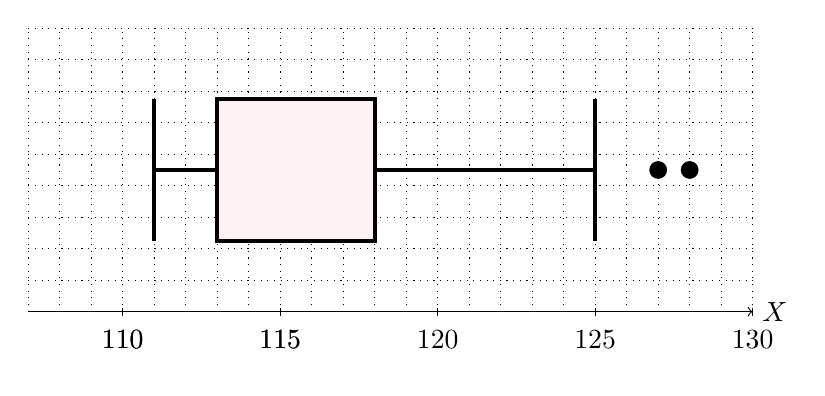
\begin{tikzpicture}[x=0.4cm,y=0.9cm]
         \draw[step=0.4cm,,dotted,color=black] (107,0) grid (130,4);
		\draw[->] (107,0) -- (130,0) node[right] {$X$} ;
		\foreach \X in {110,115,110,115,120,125,130} {
			\draw (\X,0.05cm) -- (\X,-0.05cm) node[below] {$\X\strut$};}
		\draw[ultra thick][fill=red!5] (113,1) rectangle (118,3);
		\draw[ultra thick] (111,1) -- (111,3);
		\draw[ultra thick] (111,2) -- (113,2);
		\draw[ultra thick] (118,2) -- (125,2);
		%\draw[ultra thick] (4,1) -- (4,3);
		\draw[ultra thick] (125,1) -- (125,3);
        \filldraw [black] (127, 2) circle (3pt);
        \filldraw [black] (128, 2) circle (3pt);
			\end{tikzpicture}\\
	\end{center}
\vspace{12cm}

\pagesuivante{\ref{micro}}
\newpage
\suite{\ref{micro}}

\part Vous apprenez que la plus grande observation (128) est erronée. Vous ne connaissez pas sa valeur, mais vous savez que celle-ci est plus grande que 150. Nous notons cette valeur XXX et nous savons que XXX~>~150. Le nouveau jeu de données est donc:

\begin{center}
\begin{tabular}{  c c c c c c c c }
111  &111  &111  &112  &113  &113  &113 \\
113 &114  &114  &114  &114 &115 & 116 \\
118 & 118 & 118 & 119 & 125 &127 & XXX \\
\end{tabular}
\end{center}

À partir de ce nouveau jeu de données, répondez aux questions suivantes. Nous nommons «jeu de données original» celui qui contient l'observation 128 et «nouveau jeu de données» celui qui contient l'observation XXX.

\textbf{\textit{Inscrivez «Vrai» ou «Faux» dans les cases appropriées.}}

\begin{subparts}
\subpart[3]La médiane échantillonnale du nouveau jeu de données est supérieure à celle du jeu de données orginal.


    \begin{oneparcheckboxes}
        \choice Vrai
        \correctchoice Faux
    \end{oneparcheckboxes}
\begin{solution}
La médiane est la 11\textsuperscript{e} observation ($n=21$), soit $\tilde{x}=114$ dans les deux cas. Remplacer la 21\textsuperscript{e} observation ne change pas la 11\textsuperscript{e}. Les médianes sont égales.
\end{solution}

\subpart[3] La moyenne échantillonnale du nouveau jeu de données est supérieure à celle du jeu de données original.


    \begin{oneparcheckboxes}
        \correctchoice Vrai
        \choice Faux
    \end{oneparcheckboxes}
\begin{solution}
On remplace 128 par $\text{XXX} > 150$. La somme augmente, donc $\bar{x}$ augmente aussi.
\end{solution}

\subpart[3] La variance échantillonnale du nouveau jeu de données est supérieure à celle du jeu de données orignal.


    \begin{oneparcheckboxes}
        \correctchoice Vrai
        \choice Faux
    \end{oneparcheckboxes}
\begin{solution}
La nouvelle observation est plus éloignée de la moyenne que l'ancienne (128), ce qui augmente la somme des écarts au carré et donc la variance.
\end{solution}

\end{subparts}
\end{parts}

\end{questions}
\end{document} 
